\documentclass[a4paper,12pt]{report}
\usepackage[utf8]{inputenc}
\usepackage{helvet}
\usepackage{url}
\usepackage{hyperref}
\usepackage[table]{xcolor}
\usepackage{xcolor}

\usepackage[T1]{fontenc}
\usepackage[utf8]{inputenc}
\usepackage[french]{babel}
\usepackage{amsmath}
\usepackage{amsfonts}
\usepackage{amssymb}
\usepackage{fancybox}
\usepackage{fancyhdr}
\usepackage{amsthm}
\usepackage{mathrsfs}
\usepackage{fix-cm}
\usepackage{graphicx}
\usepackage{caption}
\usepackage{subcaption}
\usepackage{textcomp}
\usepackage{lmodern}
\usepackage[tikz]{bclogo}
\usepackage{color}
\usepackage{lipsum}
\usepackage{hyperref}
\usepackage{float}
\usepackage{listings}
\usepackage{enumerate}
\usepackage[strict]{changepage}
\usepackage{ragged2e}
\usepackage{setspace}
\usepackage{array}
\usepackage{placeins}
\usepackage{hyperref}
\usepackage{titlesec}
\titleformat{\chapter}[display]
{\normalfont\huge\sc\centering}{\vspace{6.5cm}\centering\chaptertitlename \thechapter}{20pt}{\Huge}
\titlespacing*{\chapter}
{0pt}{50pt}{10pt}

\definecolor{lightgray}{gray}{0.9}

\definecolor{anti-flashwhite}{rgb}{0.95, 0.95, 0.96}
\definecolor{aliceblue}{rgb}{0.94, 0.97, 1.0}
\definecolor{beige}{rgb}{0.96, 0.96, 0.86}
\definecolor{lightapricot}{rgb}{0.99, 0.84, 0.69}
\definecolor{lightkhaki}{rgb}{0.94, 0.9, 0.55}
\definecolor{bisque}{rgb}{1.0, 0.89, 0.77}
\definecolor{arylideyellow}{rgb}{0.91, 0.84, 0.42}
\definecolor{mycolor}{RGB}{184, 206, 219}
\definecolor{colortxt}{RGB}{51,51,178}
\usepackage[left=1.9cm,right=1.4cm,top=2cm,bottom=2cm]{geometry}

\usepackage{lmodern}
\newenvironment{subs}
  {\adjustwidth{3em}{0pt}}
  {\endadjustwidth}
\usepackage{geometry}
 \geometry{
 a4paper,
 total={170mm,257mm},
 left=20mm,
 right=20mm,
 top=20mm,
 }
\setcounter{secnumdepth}{3}
\setcounter{tocdepth}{4}

\begin{document}
  
\begin{titlepage}
   \begin{sffamily}
    \begin{minipage}{0.65\textwidth}
      \begin{flushleft}
          
\includegraphics[scale=0.5]{outils-images/ens logo.png}
      \end{flushleft}
          
        
      % \end{flushleft}
      \end{minipage}
        \hspace{\fill}
    
     
    \begin{center}
     

     \vspace{1.5cm}
     \textbf{\large Université Hassan 2}\\
     \textsc{Ecole Normale Supérieure de Casablanca}\\[2.8cm]
     
     \textbf{\huge Rapport de min projet}\\[0.5cm]
     % \texttt {En vue l’obtention de la Licence Professionnelle en Ingénierie des Systèmes
     % Informatiques et Logiciels (ISIL)} :\\[0.4cm]
     
     \texttt{Sous le Thème :} \\[0.4cm]
     

\setlength{\fboxsep}{2ex} 
\setlength {\fboxrule}{2pt}
    \fbox{
      \begin{minipage}{0.9\textwidth}
       \begin{center}
          \huge \bfseries Système de détection d'intrusion
      \end{center}
    \end{minipage}
   }
     
    \begin{minipage}{0.5\textwidth}
      \begin{flushleft} \large
      \vspace{22mm}
       \textbf{Réalisé par :} \texttt{Boujrada Yassine}
       
      \end{flushleft}
    \end{minipage}
    % \begin{minipage}{0.83\textwidth}
    %   \begin{flushright} \large
    %    \vspace{3mm}
    %    \texttt{}{Pr.Lamia Ziad}
    %   \end{flushright}
    % \end{minipage}
    % \begin{minipage}{0.83\textwidth}
    %   \begin{flushright} \large
    %    \vspace{3mm}
    %    \texttt{}{Pr.Johri Mostapha}
    %   \end{flushright}
    % \end{minipage}

     \vfill
     

     {\large Année Universitaire : 2024-2025}
     
    \end{center}
   \end{sffamily}
  \end{titlepage}
  \vfill 

% \newpage
% \thispagestyle{empty} 
% \vfill
% \vfill

% \newpage
% \thispagestyle{empty}
% \hspace*{0mm}\vfill
% \chapter*{\centering Remerciements}\addcontentsline{toc}{chapter}{Remerciements}
% \begin{center}
% \indent\large\setstretch{1.25}  Tout d'abord, j’adresse ma profonde gratitude à Dieu tout-puissant qui m’a donné la force et patience pour accomplir ce modeste travail.\\
% \hspace*{0.1cm} \medskip \\
% \indent\large Il est agréable de payer une dette de gratitude au personnel de l’École Supérieure de technologie d’Essaouira et plus particulièrement à tous nos professeurs et superviseurs.\\
% \hspace*{0.2cm} \medskip \\
% \indent\large Je souhaite également exprimer mes remerciements à mon encadrante Mme.ZAHRA ASEBRIY pour sa disponibilité et tous ses précieux et sages conseils concernant les missions mentionnées dans ce rapport.\\
% \hspace*{0.2cm} \medskip \\
% \indent\large  Je tiens également à adresser mes plus sincères remerciements à mes encadrants Mr Hafid Ennaimi et Mr. Mohamed Zine qui n’ont pas cessé de m’orienter et de m’aider lors des différents suivis que j’ai eus avec eux. Ils m’ont donné les outils nécessaires pour accomplir la tâche avec plus de succès et d’intérêt.\\
% \hspace*{0.2cm} \medskip \\
% \indent\large  Enfin, je tiens à remercier tous ceux qui ont contribué directement ou indirectement à l’accomplissement de ce travail trouvent l'expression de nos remerciements les plus chaleureux.\\
% \end{center}
     
\tableofcontents
\listoffigures

\chapter*{\centering Résumé}\addcontentsline{toc}{chapter}{Résumé}
\noindent\large\setstretch{1.5}
\large Dans le cadre de notre parcour pour obtenir d'un diplôme de master en Cryptography et Cybersecurity, nous avons dû réaliser un mini projet pour ramener tous les concepts qui ont déjà été mis en œuvre .\\[0.5cm]
\large Ce projet portait sur un système de détection d’intrusion, une application essentielle dans le domaine de la sécurité informatique.\\[0.5cm]
\large Au début, je me suis concentré sur l'auto-formation sur les outils et technologies nécessaires, tels que les frameworks comme tensorflow et keras. Cette phase m'a permis de me familiariser avec les exigences du projet et de contribuer efficacement à la conception et à la mise en œuvre de la logique ainsi qu'à l'architecture de la base de données.



\chapter*{\centering Introduction générale}\addcontentsline{toc}{chapter}{Introduction générale}
\noindent\normalsize\setstretch{1.5}La conception d'applications pour gérer les processus est devenue cruciale pour les entreprises sur le marché actuel du développement de logiciels, donnant aux administrateurs la possibilité de suivre et d'améliorer les performances de l'entreprise et du personnel. \\[0.5cm]
\normalsize Simultanément, les développeurs utilisent des principes de test pour détecter et corriger les comportements logiciels problématiques, améliorant ainsi la qualité des produits.\\[0.5cm]
\normalsize Le projet décrit ici se concentre sur le développement d'un modèle de machine learning pour un système de détection d'intrusion, ou IDS, et compare différents algorithmes de machine learning, qui constituent un élément essentiel de la sécurité informatique. Pour permettre aux administrateurs de prendre des mesures préventives ou correctives, les systèmes de détection d'intrusion (IDS) sont conçus pour reconnaître et répondre aux activités suspectes ou malveillantes sur un réseau informatique.\\[0.5cm]
\normalsize Ce rapport permet d’avoir une présentation exhaustive de la démarche conduite afin de mettre à bien ce travail.
Le présent rapport est structuré comme suit :\\
\textcolor{colortxt}{Chapitre 1 :} Il porte sur le contexte général et la problématique du travail réalisé.\\
\textcolor{colortxt}{Chapitre 2 :} Il appuie sur exportation, l'importation, la manipulation et la visualisation des données.\\
\textcolor{colortxt}{Chapitre 3 :} Il présente la partie d'apprentissage et evaluation les résultat de modéle.\\[0.5cm]
Au terme de ce rapport une conclusion avec perspectives est donnée qui synthétise tout le travail réalisé



\renewcommand{\chaptername}{Chapter}
\chapter{CONTEXTE GÉNÉRALE SUR IDS}

\newpage
\pagestyle{plain} 
\section{Introduction}
\noindent \normalsize Ce chapitre sera une présentation du contexte générale  ainsi que la problématique abordée.
\section{Qu'est-ce que systèmes de détection d’intrusion (IDS)}
\noindent \normalsize Un système de détection des intrusions (IDS) \cite{axelsson2000intrusion} est une application qui surveille le trafic réseau et recherche les menaces connues et les activités suspectes ou malveillantes. L’IDS envoie des alertes aux équipes informatiques et de sécurité lorsqu’il détecte des risques et des menaces de sécurité.
\normalsize La plupart des solutions IDS surveillent et signalent simplement les activités et le trafic suspects lorsqu’elles détectent une anomalie.\\[0.5cm]
\begin{figure}[H]
\centering
 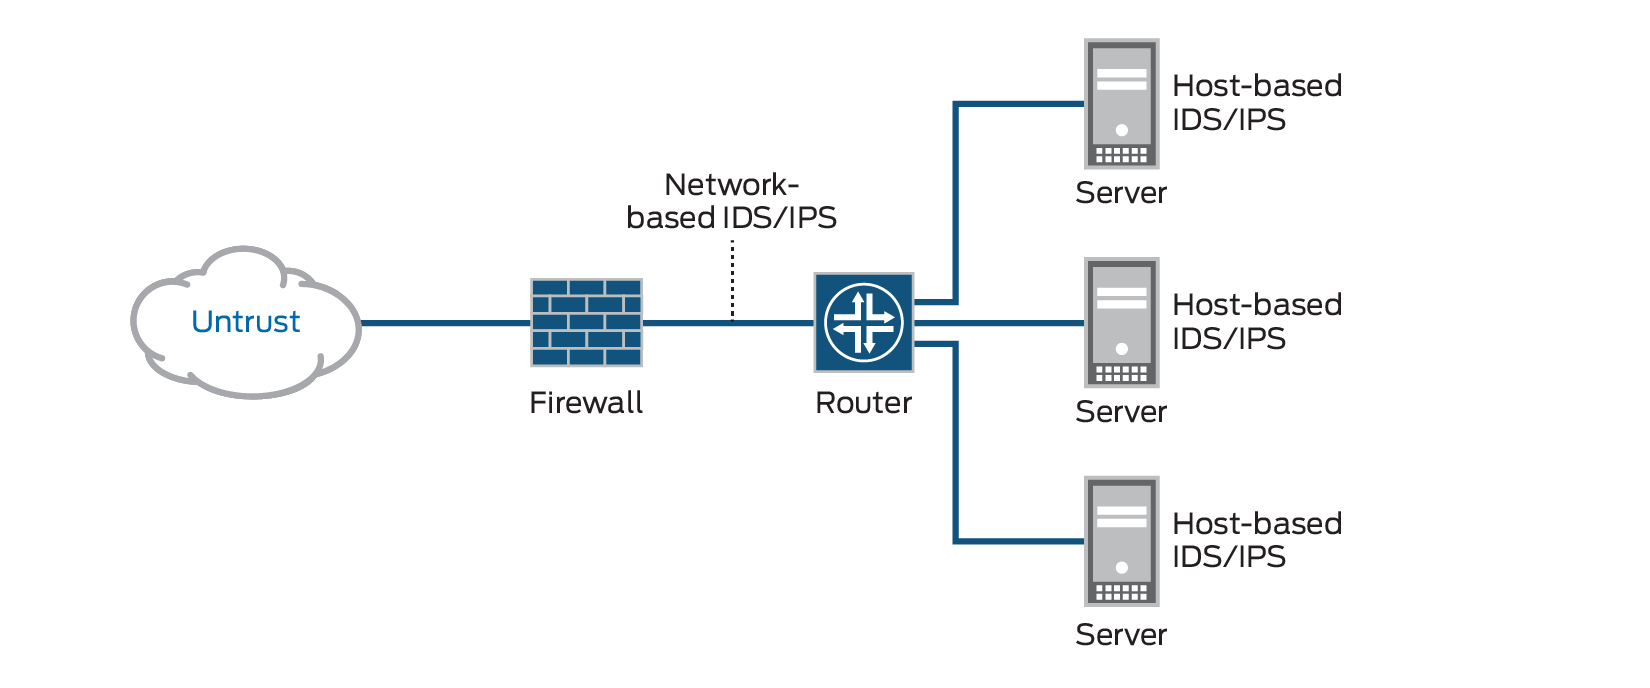
\includegraphics[scale=0.9]{outils-images/ids_schem.jpg}
\caption{Schéma de IDS/IP}
\end{figure}
\normalsize \noindent Les outils IDS sont généralement des applications logicielles qui s’exécutent sur le matériel des organisations ou en tant que solution de sécurité réseau. Il existe également des solutions IDS basées sur le cloud qui protègent les données, les ressources et les systèmes des organisations dans leurs environnements et déploiements cloud.

\section{Types de systèmes de détection d’intrusion (IDS)}
\noindent \normalsize Les types courants de systèmes de détection des  intrusions (IDS) comprennent :
\begin{itemize}
    \item Système de détection des intrusions réseau (NIDS) : une solution NIDS est déployée à des points stratégiques du réseau d’une organisation pour surveiller le trafic entrant et sortant. Cette approche IDS surveille et détecte le trafic malveillant et suspect entrant et sortant de tous les appareils connectés au réseau.
    \item Système de détection d’intrusion hôte (HIDS) : un système HIDS est installé sur des appareils individuels connectés à Internet et au réseau interne d’une organisation. Cette solution peut détecter les paquets provenant de l’intérieur de l’entreprise et le trafic malveillant supplémentaire qu’une solution NIDS ne peut pas détecter.\\[0.1cm]
    \item Système de détection des intrusions (SIDS) basé sur les signatures : une solution SIDS surveille tous les paquets sur le réseau d’une organisation et les compare aux signatures d’attaque sur une base de données de menaces connues.\\[0.1cm]
    \item Système de détection des intrusions (SIDA) basé sur les anomalies : cette solution surveille le trafic sur un réseau et le compare à une ligne de base prédéfinie considérée comme « normale ». Il détecte les activités et comportements anormaux sur le réseau, y compris la largeur de bande appareils, les ports et les protocoles.
\end{itemize}


\section{Méthode de détection de IDS}
\normalsize \noindent \textcolor{colortxt}{Méthode basée sur les signatures :} IDS basé sur les signatures détecte les attaques sur la base de modèles spécifiques tels que le nombre d'octets ou le nombre de 1 ou le nombre de 0 dans le trafic réseau. Il détecte également sur la base de la séquence d'instructions malveillantes déjà connue et utilisée par le logiciel malveillant. Les modèles détectés dans l'IDS sont appelés signatures. L'IDS basé sur les signatures peut facilement détecter les attaques dont le modèle (signature) existe déjà dans le système, mais il est assez difficile de détecter les nouvelles attaques de logiciels malveillants car leur modèle (signature) n'est pas connu.\\[0.2cm]
\normalsize \noindent \textcolor{colortxt}{Méthode basée sur les anomalies :} l'IDS basé sur les anomalies a été introduit pour détecter les attaques de logiciels malveillants inconnus à mesure que de nouveaux logiciels malveillants se développent rapidement. Dans l'IDS basé sur les anomalies, l'apprentissage automatique est utilisé pour créer un modèle d'activité fiable et tout ce qui arrive est comparé à ce modèle et est déclaré suspect s'il n'est pas trouvé dans le modèle. La méthode basée sur l'apprentissage automatique a une propriété mieux généralisée par rapport à l'IDS basé sur les signatures, car ces modèles peuvent être formés en fonction des applications et des configurations matérielles.
\section{Conclusion}
\noindent \normalsize Au cours de ce chapitre, j'ai présenté le contexte général sur le topic, les types, et méthode de détection qui selon on peut utiliser pour notre modéle. 



\renewcommand{\chaptername}{Chapter}
\chapter{Exporter DataSet}

\newpage
\pagestyle{plain} 
\section {Introduction}
\noindent\normalsize Dans le domaine du Machine Learning, l’efficacité de votre modèle dépend de la qualité de vos jeux de données (DataSet). Ainsi, l'exportation du DataSet est une étape cruciale. Pour cela, il existe des bibliothèques utilisées pour manipuler les données, et dans notre cas, nous avons utilisé Pandas.
\noindent\normalsize Pour notre DataSet, nous avons utilisé dans ce projet un ensemble de données provenant de \textcolor{colortxt}{Kaggle}, d'une taille de 1,2 Go. Voici un exemple d'échantillon : \href{https://www.kaggle.com/datasets/hassan06/nslkdd}{Exportation de DataSet de taille 55.87 MB}.


\section {Les informations sur les données}
\noindent\normalsize Pour obtenir des informations sur nos données, nous commençons par importer le fichier, puis nous utilisons la fonction ".info()".
\begin{figure}[H]
\centering
 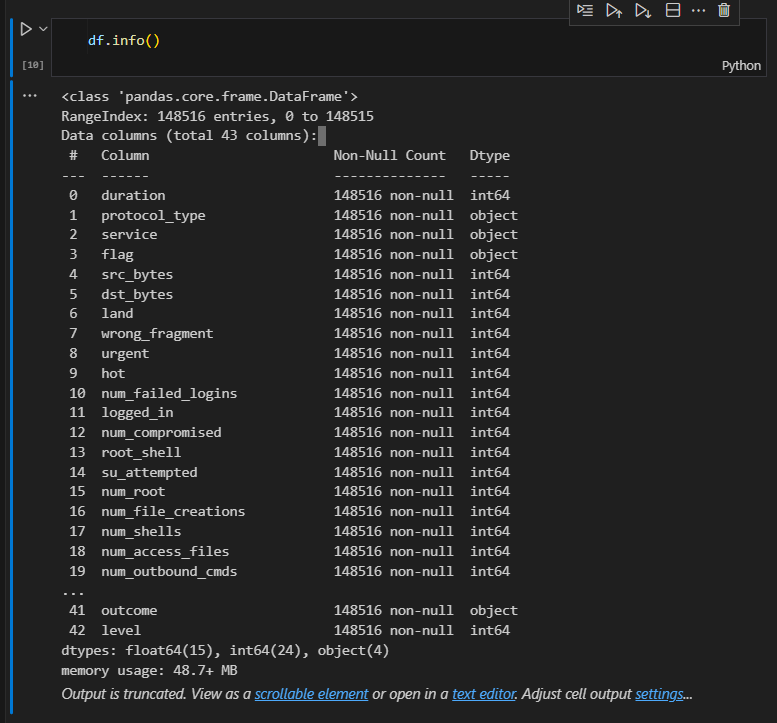
\includegraphics[scale=0.9]{outils-images/data1.png}
\caption{Informations sur les colonnes du dataset}
\end{figure}
\noindent\normalsize Ensuite, pour déterminer s'il existe des valeurs nulles à éliminer, nous utilisons la fonction ".isnull().sum()".
\begin{figure}[H]
\centering
 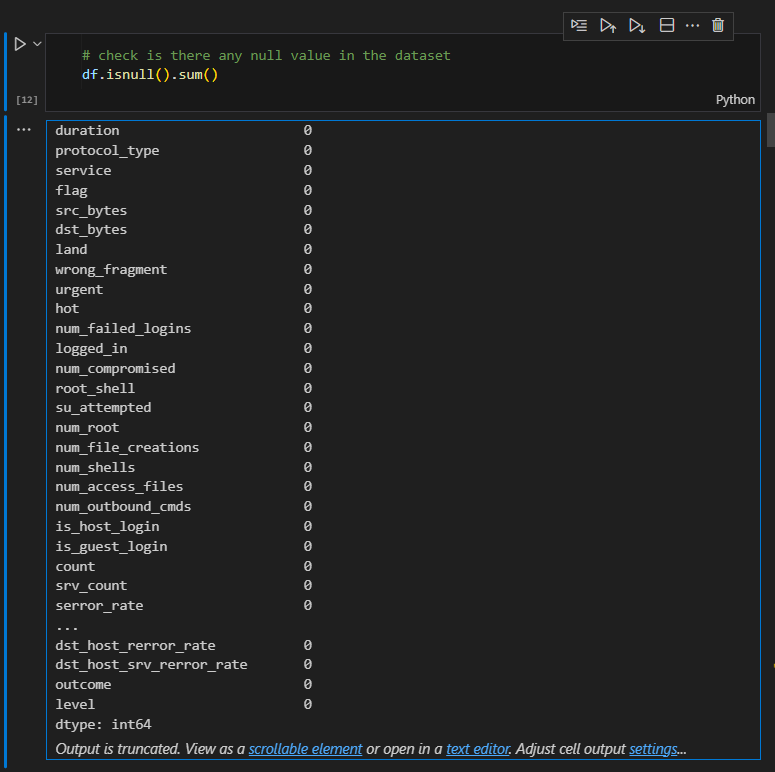
\includegraphics[scale=0.9]{outils-images/data3.png}
\caption{les valeurs nulles en dataset}
\end{figure}
\noindent\normalsize Ensuite, pour les types d'attaques que nous devons traiter dans nos données,

\begin{figure}[H]
    \centering
    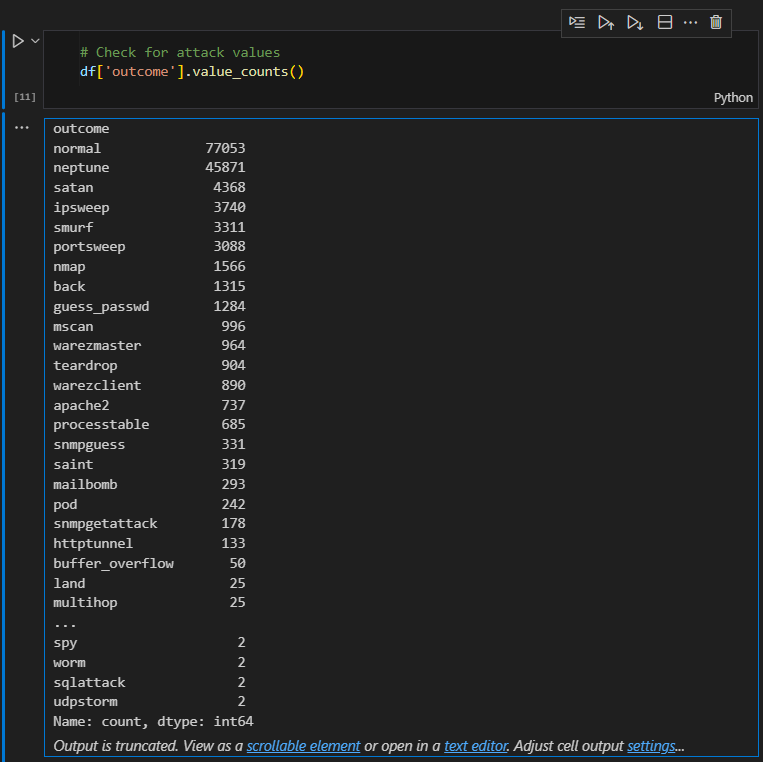
\includegraphics[scale=0.9]{outils-images/data2.png}
    \caption{Les types d'attaques en dataset}
    \label{fig:types_attaques}
\end{figure}

\noindent\normalsize Comme nous l'observons dans la figure \ref{fig:types_attaques}, il existe plusieurs types d'attaques. Afin de simplifier le travail, nous pouvons classifier tous ces résultats en deux labels : "normale" et "attaque".
\begin{figure}[H]
    \centering
    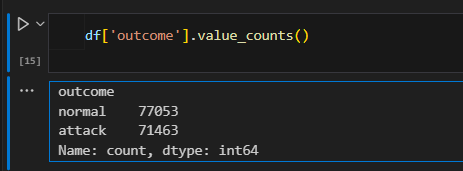
\includegraphics[scale=0.9]{outils-images/data5.png}
    \caption{Les outcomes en dataset}
\end{figure}
\noindent\normalsize Pour une meilleure visualisation, on utilise Matplotlib pour afficher les données sous forme de graphiques.
\begin{figure}[H]
    \centering
    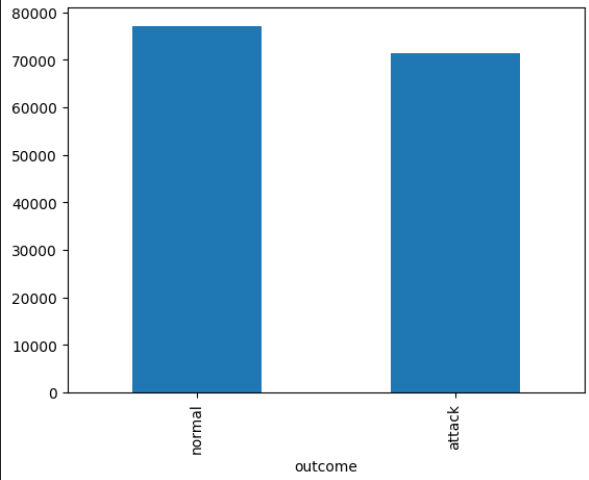
\includegraphics[scale=0.9]{outils-images/graphs/g1.png}
    \caption{graphique des outcomes en dataset}
\end{figure}


\section {Data Visualization}
\noindent\normalsize La visualisation des données\cite{scikit-learn-visualization} est une composante essentielle de l'analyse et de la compréhension des données dans de nombreux domaines, notamment la science des données, la recherche, les affaires et plus encore.\\[0.5cm]
\noindent\normalsize Nous commençons par examiner le graphique ci-dessus, qui est un diagramme circulaire contenant deux sous-graphiques distincts. Le premier sous-graphique résume l'utilisation des protocoles, en mettant en évidence les nombres relatifs de protocoles tels que TCP, UDP et ICMP. Le deuxième sous-graphique vise à évaluer l'équilibre des valeurs de sortie (outcomes) afin de prévenir les problèmes potentiels lors de la phase d'entraînement, comme overfitting
\begin{figure}[H]
\centering
 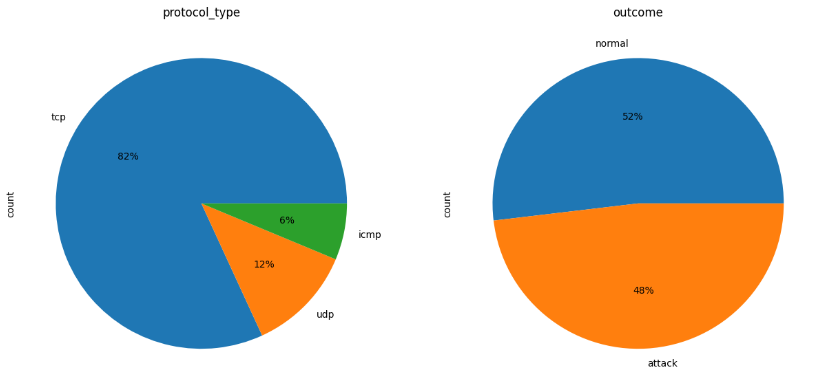
\includegraphics[scale=0.9]{outils-images/graphs/g2.png}
\caption{les types de protocoles et sortie en dataset}
\end{figure}
\noindent\normalsize Pour visualiser la répartition des différentes attaques en fonction du type de protocole dans l'ensemble de données, on a
\begin{figure}[H]
\centering
 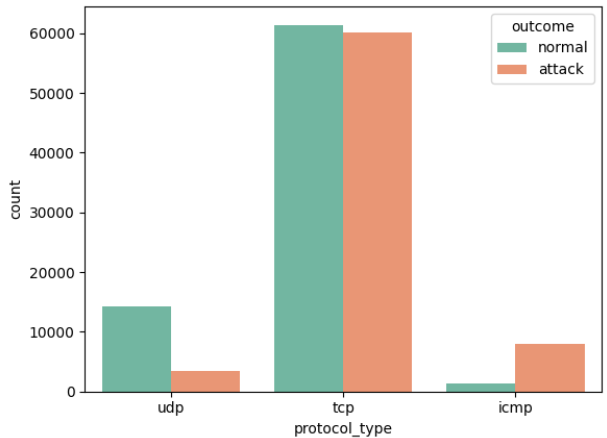
\includegraphics[scale=0.9]{outils-images/graphs/g3.png}
\caption{les types de protocoles en fonction d'attaque}
\end{figure}
\noindent\normalsize Il y'a un attribut particulièrement en notre dataset qui est interessent "logged in" car il indique si un utilisateur est actuellement connecté à un système ou à une plateforme. Cette information est souvent utilisée pour suivre et analyser le comportement des utilisateurs, notamment dans les systèmes informatiques, les applications en ligne
\begin{figure}[H]
\centering
 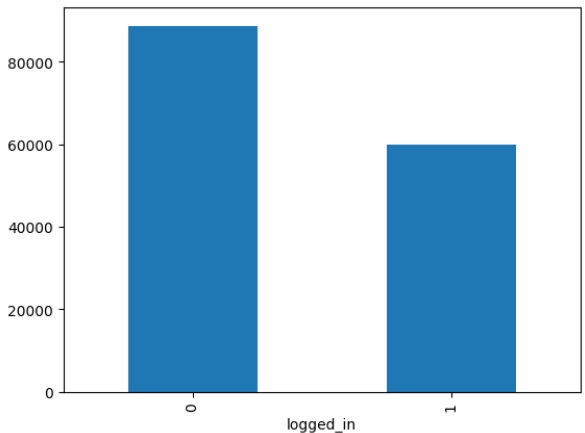
\includegraphics[scale=0.9]{outils-images/graphs/g4.png}
\caption{logged in column}
\end{figure}

\section {Data Correlation}
\noindent\normalsize Pour simplifier \cite{hair2019multivariate}, il s'agit de la mesure dans laquelle une variable change par rapport à une autre. Il mesure la force et la direction de la relation entre deux ou plusieurs variables
nous allons vérifier la corrélation entre les variables de notre ensemble de données pour voir lesquelles ne peuvent pas être utilisées dans notre modèle.
\begin{itemize}
    \item 1 : indique une relation linéaire positive parfaite.
    \item 0 : indique aucune relation linéaire.
    \item -1 : indique une relation linéaire négative parfaite
\end{itemize}
\noindent\normalsize Mais après avoir travaillé sur cet attribut, nous avons besoin d'utiliser des méthodes pour encoder les variables qui sont de type chaîne de caractères. Dans notre ensemble de données, nous avons des attributs tels que "service", "flag", "type de protocole" et "outcome". Pour cela, nous utilisons le labelEncoder, qui est une technique largement utilisée pour attribuer des valeurs numériques aux variables de catégorie. 
\begin{figure}[H]
\centering
 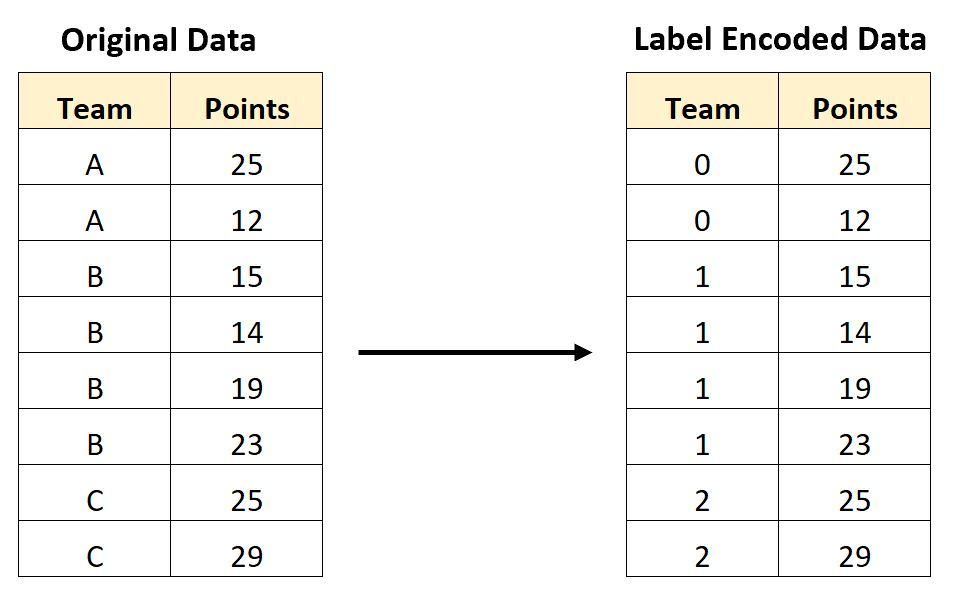
\includegraphics[scale=0.9]{outils-images/data6.jpg}
\caption{exemple de Label Encoder}
\end{figure}
\noindent\normalsize Chaque catégorie de la variable reçoit un identifiant numérique distinct par labelEncoder, permettant une représentation numérique des catégories dans notre analyse.
\noindent\normalsize Alors après avoir calculé la corrélation de chaque attribut de notre ensemble de données avec les autres, nous obtenons comme résultat final ce graphique.
\begin{figure}[H]
\centering
 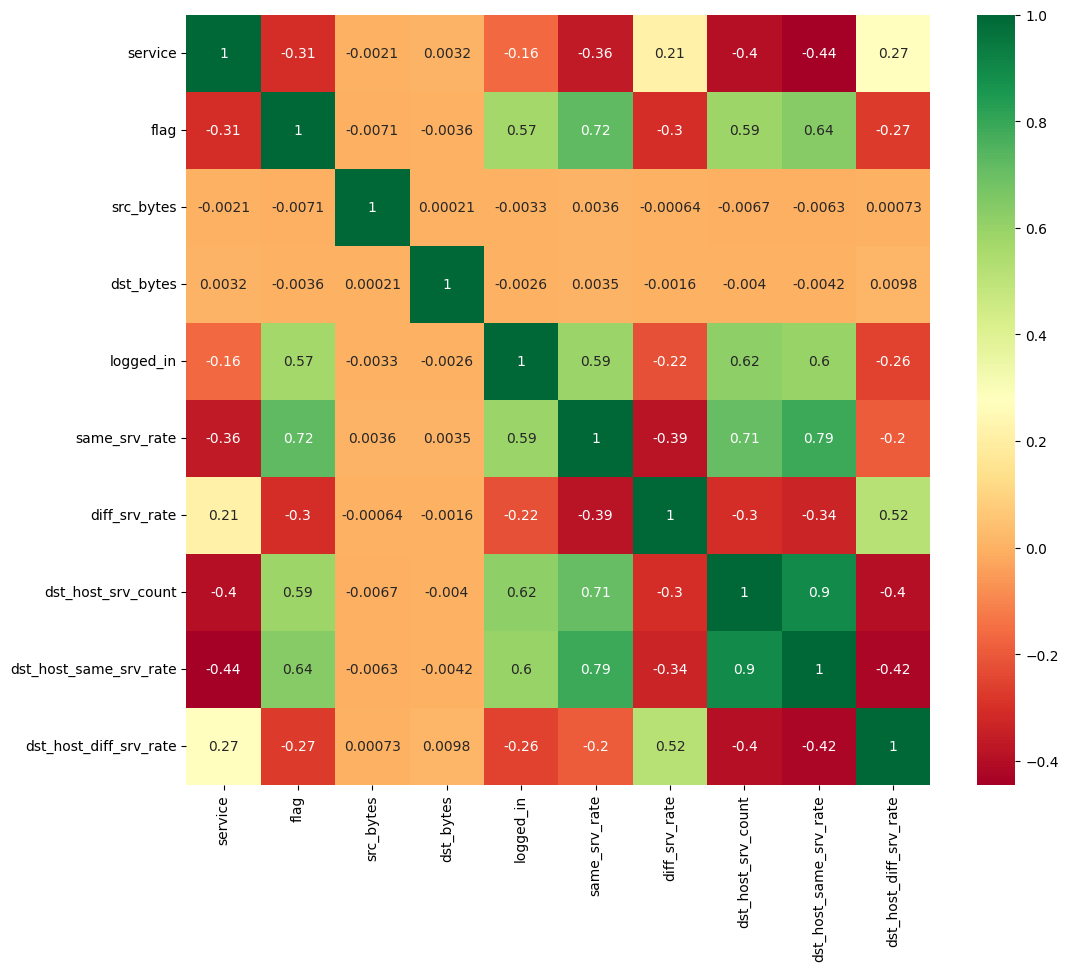
\includegraphics[scale=0.6]{outils-images/graphs/g5.png}
\caption{Correlation de chaque attribut avec les autres attributes}
\end{figure} 

\section{Conclusion}
\noindent\normalsize Après avoir normalisé nos données et réalisé les visualisations nécessaires, la prochaine étape consiste à travailler sur le modèle et à choisir le bon algorithme pour notre problématique.



\renewcommand{\chaptername}{Chapter}
\chapter{Model D'apprentissage}

\newpage
\pagestyle{plain} 
\section{Introduction}
\noindent \normalsize 
Ce chapitre présente tout ce qui concerne notre modèle, notamment la séparation de notre ensemble de données en ensembles d'apprentissage et de test, ainsi que l'analyse de chaque algorithme utilisée.


\section{Fractionnement des données}
\noindent \normalsize Pour cette problématique, nous nous concentrons sur un problème de classification, une tâche fondamentale en apprentissage automatique. La classification consiste à attribuer des étiquettes ou des catégories à des données en fonction de leurs caractéristiques, permettant ainsi de distinguer différentes classes ou catégories. En fonction des données fournies à notre modèle, celui-ci sera en mesure de prédire si une observation est considérée comme normale ou si elle constitue une attaque.\\[0.2cm]
\noindent \normalsize Donc attribut que nous devons prédire est désigné sous le nom de \textcolor{colortxt}{Outcome}. Pour séparer les attributs et les stocker dans différentes variables, nous réalisons une opération de partitionnement de notre ensemble de données.
\begin{figure}[H]
\centering
 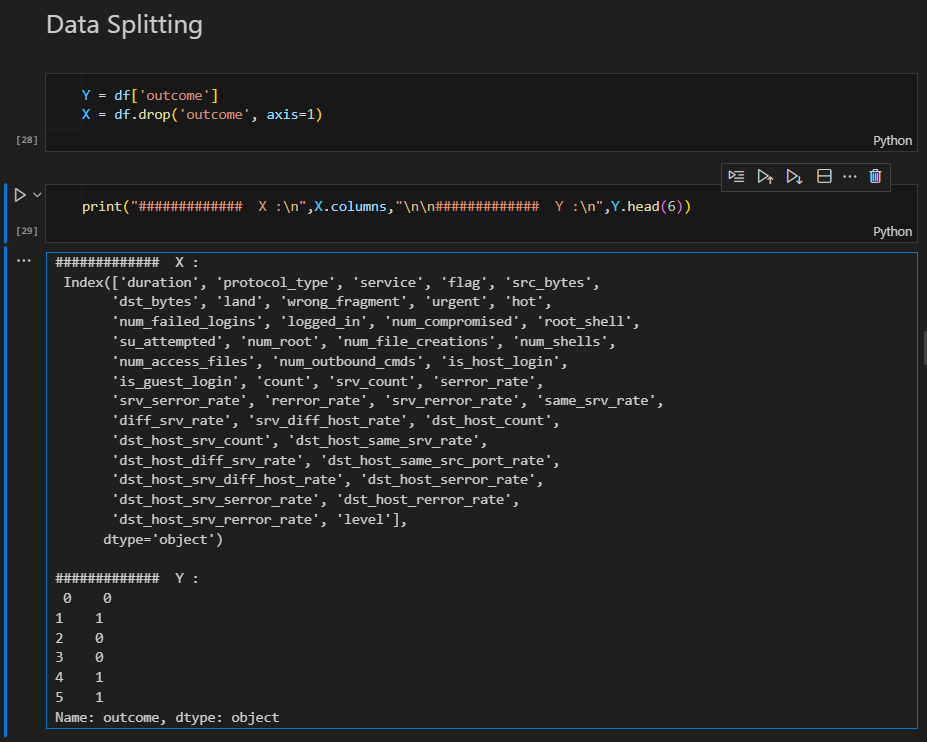
\includegraphics[scale=0.7]{outils-images/data7.png}
\caption{Séparer les attributes}
\end{figure} 
\noindent \normalsize Après cette étape, nous avons utilisé deux méthodes de division de données afin de les comparer et de déterminer si la méthode utilisée influence l'efficacité du modèle. Ces méthodes sont la 
\textcolor{colortxt}{Train Test Split} et \textcolor{colortxt}{Cross Validation} .

\subsection{Train Test Split}
\noindent \normalsize Une fois la fonction train test split\cite{ sklearn-train-test-split} définie, elle renvoie un ensemble train et un ensemble test. Ce splitting des données permet d’évaluer un modèle de Machine Learning sous deux angles différents.Le modèle est entraîné sur l’ensemble train renvoyé par la fonction. Puis ses capacités prédictives sont évaluées sur l’ensemble test renvoyé par la fonction. Plusieurs métriques peuvent être utilisées pour cette évaluation.
\begin{figure}[H]
\centering
 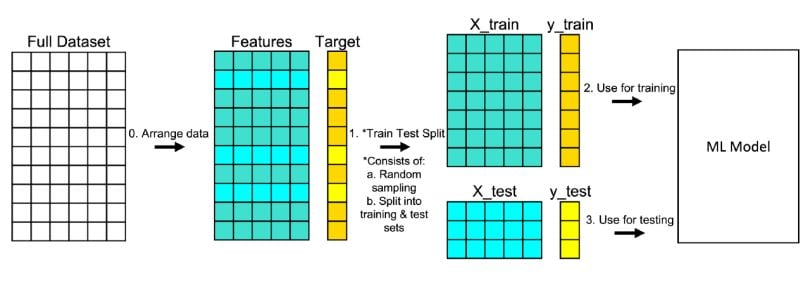
\includegraphics[scale=0.6]{outils-images/data8.jpg}
\caption{Schéma de train test split}
\end{figure} 
\noindent \normalsize Dans le cas d’une régression linéaire, le coefficient de détermination, la RMSE et la MAE sont privilégiés. Dans le cas d’une classification, l’accuracy, la précision, le recall et le F1-score sont privilégiés. Ces scores sur l’ensemble test permettent donc de déterminer si le modèle est performant et à quel point il doit être amélioré avant de pouvoir prédire sur un nouveau dataset.
Les ensembles train et test renvoyés par la fonction train test split jouent aussi un rôle essentiel dans la détection d’overfitting ou d’underfitting.
Pour notre code :
\begin{figure}[H]
\centering
 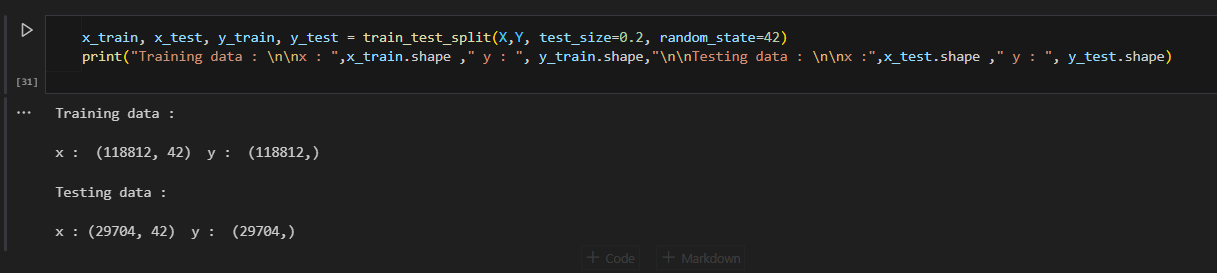
\includegraphics[scale=0.7]{outils-images/data9.png}
\caption{implémetation de train test split en notre code}
\end{figure} 

\subsection{Cross Validation ou k-Folds}
\noindent \normalsize Facile à comprendre et très populaire auprès des professionnels, la technique K-Folds\cite{scikit-learn}, propose généralement un modèle moins biaisé que les autres méthodes qui existe. La principale raison est qu'elle permet de s'assurer que toutes les observations du jeu de données original puissent apparaître dans l'ensemble d'entraînement, mais aussi dans l'ensemble utilisé pour le test. Dans la situation où les données d'input sont limitées, c'est l'une des meilleures solutions à considérer.
\begin{figure}[H]
\centering
 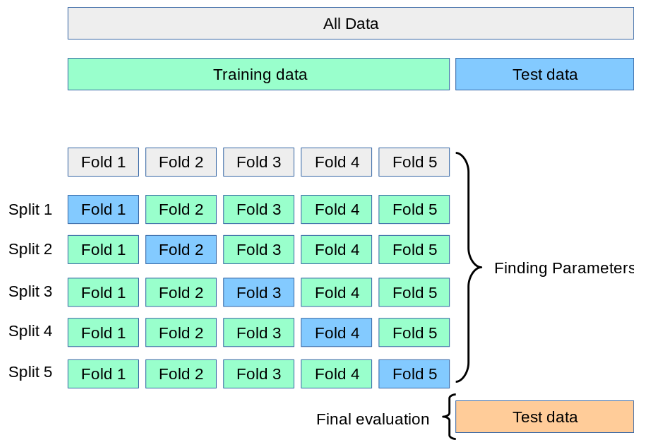
\includegraphics[scale=0.8]{outils-images/data11.png}
\caption{Schéma de Cross Validation}
\end{figure} 
\noindent \normalsize Pour commencer, on effectue d'abord une séparation de l'ensemble de données de façon aléatoire en K folds. Un paramétrage unique dénommé « K » est inséré dans la procédure, se référant au nombre de groupe dans lequel l'échantillon sera réparti. K doit avoir une valeur ni trop basse ni trop haute. La plupart du temps, on choisira une valeur qui se situe entre 5 et 10 selon la taille du dataset. Dans le cas où K=10, cela implique qu'il faut diviser le dataset en 10 parties.\\[0.2cm]

\noindent \normalsize Plus la valeur K est élevée, moins le modèle risque d'être biaisé. Sans oublier qu'une variance trop large peut amener à un surajustement. Avec une valeur plus basse, l'approche rejoint simplement la méthode Train-Test Split.
En notre code :
\begin{figure}[H]
\centering
 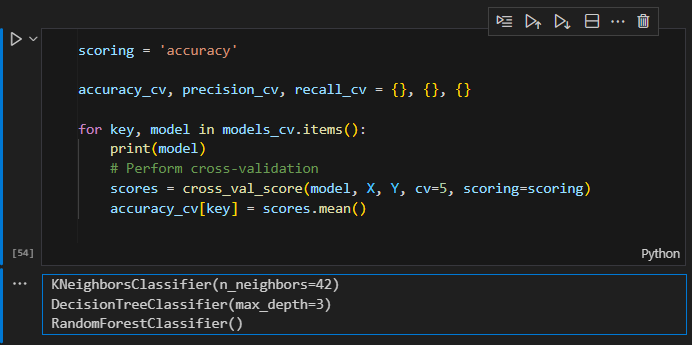
\includegraphics[scale=0.9]{outils-images/data10.png}
\caption{implémetation de Cross Validation en notre code}
\end{figure} 

\section{Modeling}
\subsection{Algorithmes d'apprentissage automatique}
\noindent \normalsize En notre code, nous travaillons avec quatre algorithmes de classification : la régression logistique, la méthode des k plus proches voisins (KNN), les arbres de décision et la forêt d'arbres aléatoires (Random Forest).
\subsubsection{Phase Entraînement }
\textcolor{colortxt}{la régression logistique :}\cite{hosmer2013applied}
Ce type de modèle statistique (également appelé modèle logit) est souvent utilisé pour la classification et l'analyse prédictive. La régression logistique estime la probabilité qu'un événement se produise, comme avoir voté ou non, sur la base d'un ensemble de données donné de variables indépendantes. Puisque le résultat est une probabilité, la variable dépendante est limitée entre 0 et 1. Dans la régression logistique, une transformation logit est appliquée aux probabilités, c'est-à-dire la probabilité de succès divisée par la probabilité d'échec. Ceci est également communément appelé log des cotes, ou logarithme naturel des cotes, et cette fonction logistique est représentée par les formules suivantes :
\begin{figure}[H]
\centering
 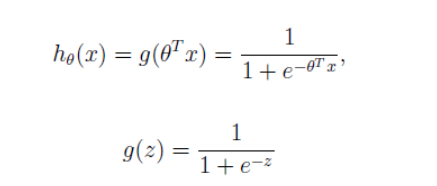
\includegraphics[scale=0.9]{outils-images/data12.png}
\caption{formule mathématique de régression logistique}
\end{figure}

\textcolor{colortxt}{k plus proches voisins (KNN) :}
\noindent \normalsize également connu sous le nom de KNN ou k-NN, est un classificateur d'apprentissage supervisé non paramétrique, qui utilise la proximité pour effectuer des classifications ou des prédictions sur le regroupement d'un point de données individuel. Bien qu'il puisse être utilisé pour des problèmes de régression ou de classification, il est généralement utilisé comme algorithme de classification, partant de l'hypothèse que des points similaires peuvent être trouvés les uns à proximité des autres.
\begin{figure}[H]
\centering
 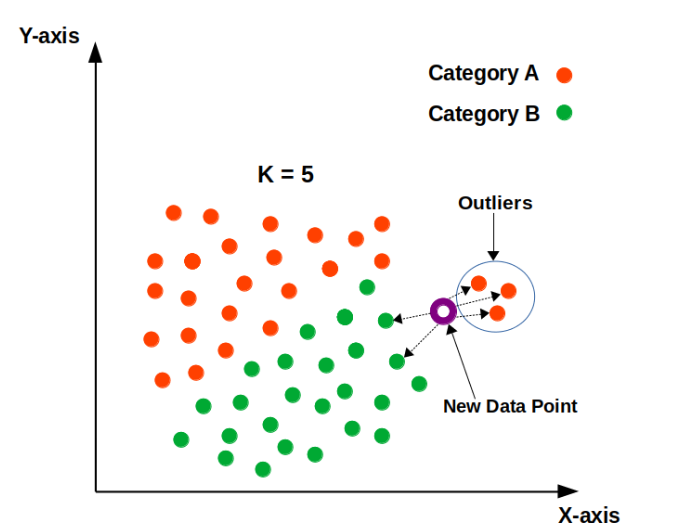
\includegraphics[scale=0.9]{outils-images/data13.png}
\caption{Schéma de k plus proches voisins}
\end{figure}

\textcolor{colortxt}{L'arbre de décision :}
\noindent \normalsize est l'outil de classification et de prédiction le plus puissant et le plus populaire. Un arbre de décision est une structure arborescente de type organigramme, dans laquelle chaque nœud interne désigne un test sur un attribut, chaque branche représente un résultat du test et chaque nœud feuille (nœud terminal) contient une étiquette de classe.
\begin{figure}[H]
\centering
 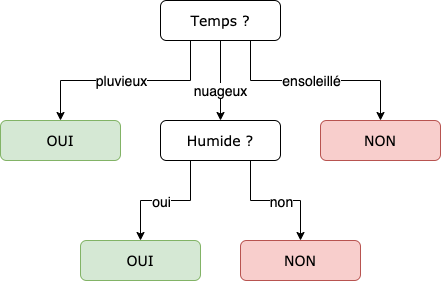
\includegraphics[scale=0.7]{outils-images/data14.jpg}
\caption{Schéma d'arbre de décision}
\end{figure}

\textcolor{colortxt}{la forêt d’arbres aléatoires (Random Forest) :}
\noindent \normalsize est l'outil de classification et de prédiction le plus puissant et le plus populaire. Un arbre de décision est une structure arborescente de type organigramme, dans laquelle chaque nœud interne désigne un test sur un attribut, chaque branche représente un résultat du test et chaque nœud feuille (nœud terminal) contient une étiquette de classe.
\begin{figure}[H]
\centering
 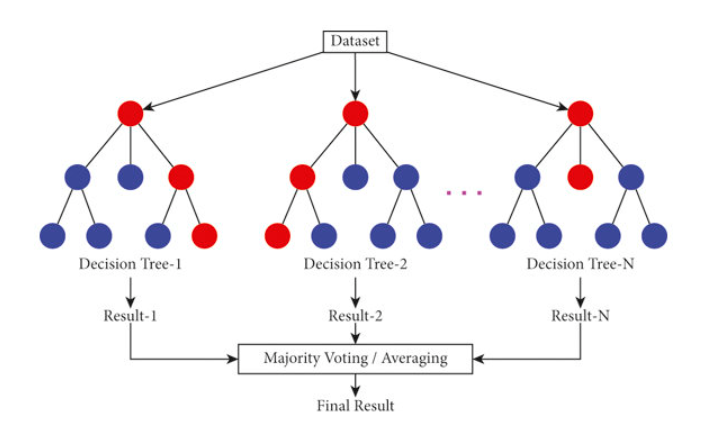
\includegraphics[scale=0.9]{outils-images/data15.png}
\caption{Schéma de Random Forest}
\end{figure}

\noindent \normalsize Pour implémenter ces algorithmes dans notre code, nous commençons par initialiser chacun d'entre eux.
\begin{figure}[H]
\centering
 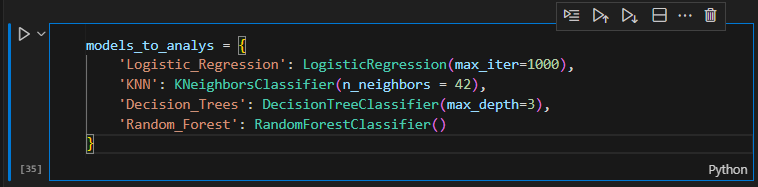
\includegraphics[scale=0.9]{outils-images/data16.png}
\caption{initialiser chaque algorithme}
\end{figure}
\noindent \normalsize Après avoir entraîné ces algorithmes avec les données d'entraînement et calculé leur exactitude (accuracy), leur précision (precision) et leur rappel (recall) pour chaque algorithme. 
ca par Train Test Split dataset :
\begin{figure}[H]
\centering
 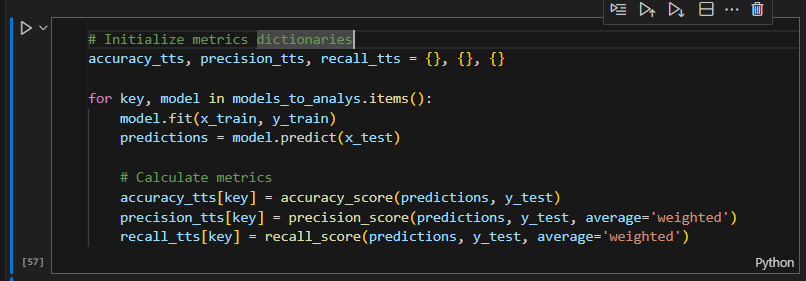
\includegraphics[scale=0.9]{outils-images/data17.png}
\caption{Entraînement ces algorithme par train test datasplit}
\end{figure}
et pour Cross Validation :
\begin{figure}[H]
\centering
 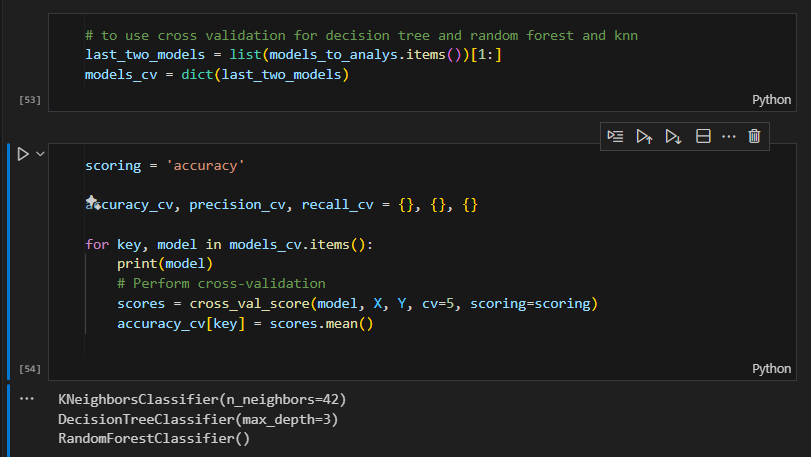
\includegraphics[scale=0.9]{outils-images/data18.png}
\caption{Entraînement ces algorithme par Cross Validation méthode}
\end{figure}

\subsubsection{Phase Evaluation }
\noindent \normalsize Enfin, dans cette partie, nous pouvons évaluer chaque algorithme que nous avons utilisé et répondre à la question de savoir si les méthodes de fractionnement des données peuvent affecter l'efficacité de notre modèle.Pour cela, nous calculons l'exactitude (accuracy), le rappel (recall) et la précision (precision) pour chaque algorithmes.
\begin{figure}[H]
\centering
 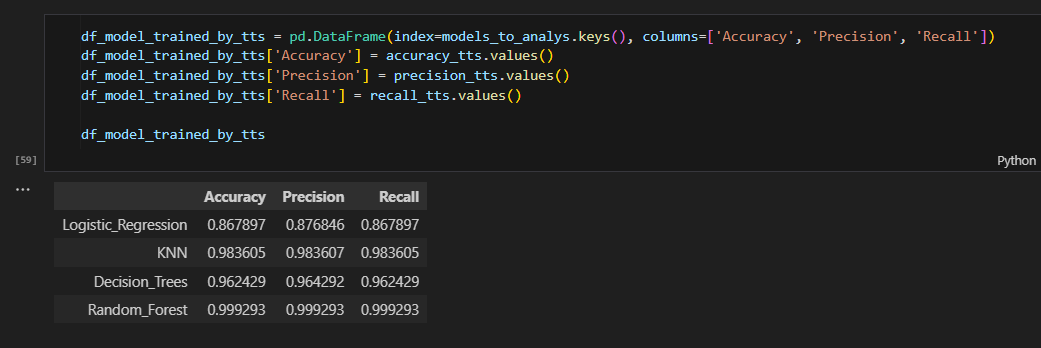
\includegraphics[scale=0.8]{outils-images/data19.png}
\caption{Evaluation de ces algorithme}
\end{figure}

\noindent \normalsize pour rendre le résultat présentable, nous le montrons sous forme de graphique
\begin{figure}[H]
\centering
 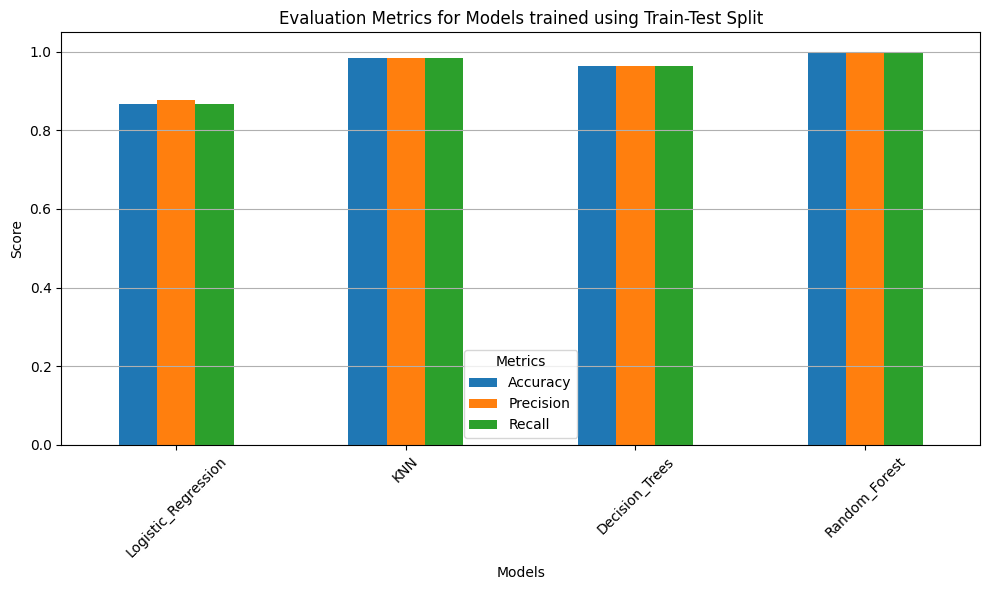
\includegraphics[scale=0.6]{outils-images/data20.png}
\caption{Métriques d'évaluation pour les modèles formés à l'aide de Train-Test Split}
\end{figure}

\noindent \normalsize Nous utilisons également la matrice de confusion pour évaluer les performances de chaque algorithme qui est une représentation tabulaire qui permet de visualiser les performances d'un modèle de classification. Elle compare les valeurs réelles des données avec les prédictions du modèle, en classifiant les prédictions en quatre catégories : vrai positif (TP), vrai négatif (TN), faux positif (FP) et faux négatif (FN) .
\begin{figure}[H]
\centering
 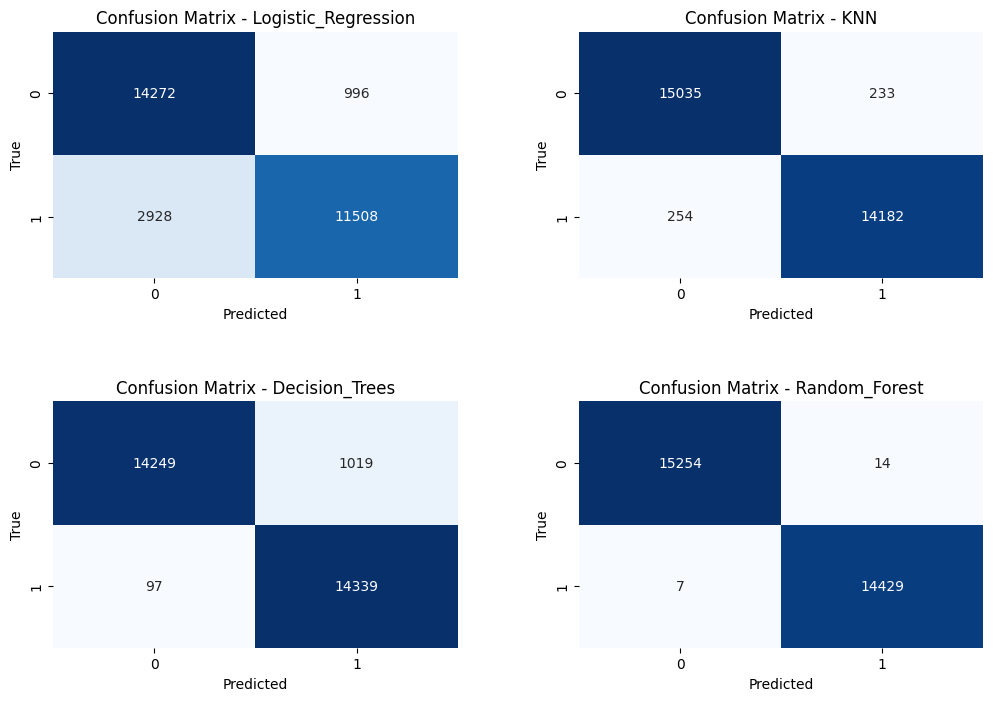
\includegraphics[scale=0.6]{outils-images/graphs/g6.png}
\caption{Matrice de confusion}
\end{figure}

\noindent \normalsize Pour répondre à la question de savoir si les méthodes de fractionnement des données (Data Splitting) peuvent affecter l’efficacité de notre modèle, nous présentons les résultats sur ce graphe.
\begin{figure}[H]
\centering
 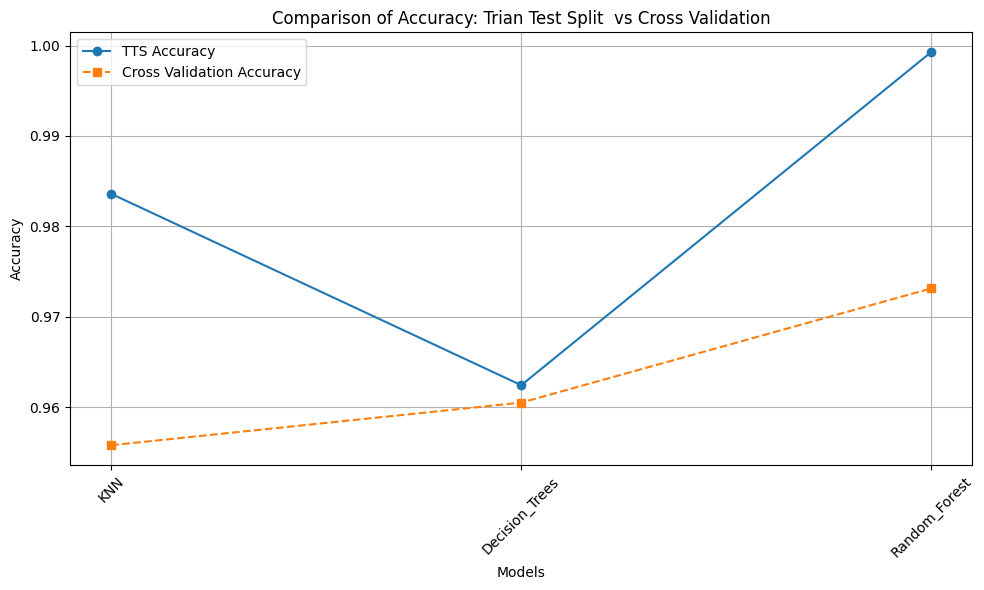
\includegraphics[scale=0.6]{outils-images/graphs/g7.png}
\caption{Comparaison de Accuracy : Trian Test Split  vs Cross Validation}
\end{figure}
\noindent \normalsize Dans le graphe, nous mettons en évidence la méthode choisie pour le fractionnement des données qui joue un rôle crucial dans l'évaluation de notre modèle.

\subsection{Deep Learning  : }
\noindent \normalsize Les réseaux de neurones, également appelés réseaux de neurones artificiels (ANN) ou réseaux de neurones simulés (SNN), sont un sous-ensemble de l'apprentissage automatique et sont au cœur des algorithmes d'apprentissage profond. Leur nom et leur structure sont inspirés du cerveau humain, imitant la façon dont les neurones biologiques se communiquent les uns aux autres. Les réseaux de neurones artificiels (ANN) sont constitués d'une couche de nœuds contenant une couche d'entrée, une ou plusieurs couches cachées et une couche de sortie. Chaque nœud, ou neurone artificiel, se connecte à un autre et possède un poids et un seuil associés. Si la sortie d'un nœud individuel est supérieure à la valeur seuil spécifiée, ce nœud est activé et envoie des données à la couche suivante du réseau. Sinon, aucune donnée n’est transmise à la couche suivante du réseau.
\begin{figure}[H]
\centering
 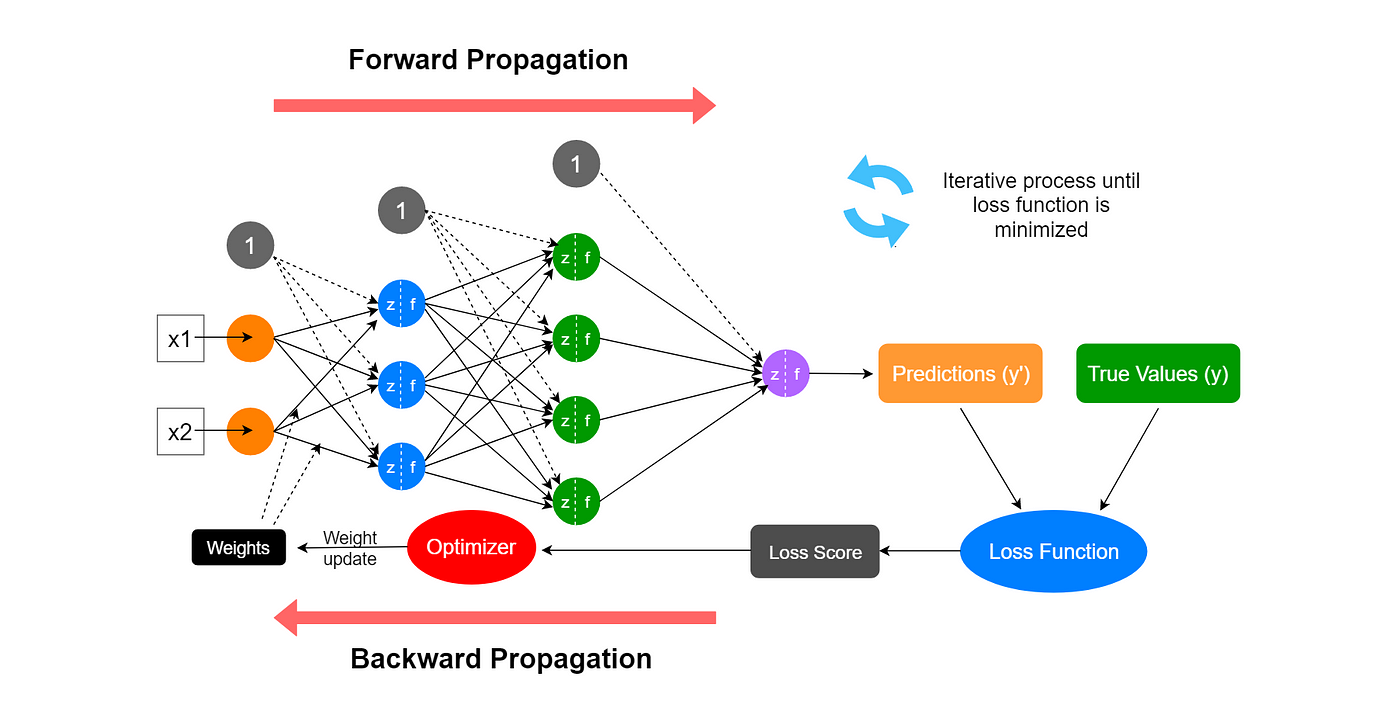
\includegraphics[scale=0.35]{outils-images/data28.png}
\caption{Exemple d'un réseau de neurone}
\end{figure}

\noindent \normalsize Ainsi, pour l'architecture de notre modèle, nous utilisons un réseau de neurones séquentiel avec plusieurs couches de neurones denses. Chaque couche est suivie d'une couche d'abandon, qui désactive certains neurones pendant l'entraînement pour éviter le surapprentissage. Le modèle commence par une petite couche dense, puis passe par des couches qui s'élargissent progressivement avant de se rétrécir à nouveau vers la sortie. Quant à la régularisation, nous appliquons des pénalités aux poids et activations de chaque couche pour éviter que le modèle ne soit surajusté aux données d'entraînement. 
\begin{figure}[H]
\centering
 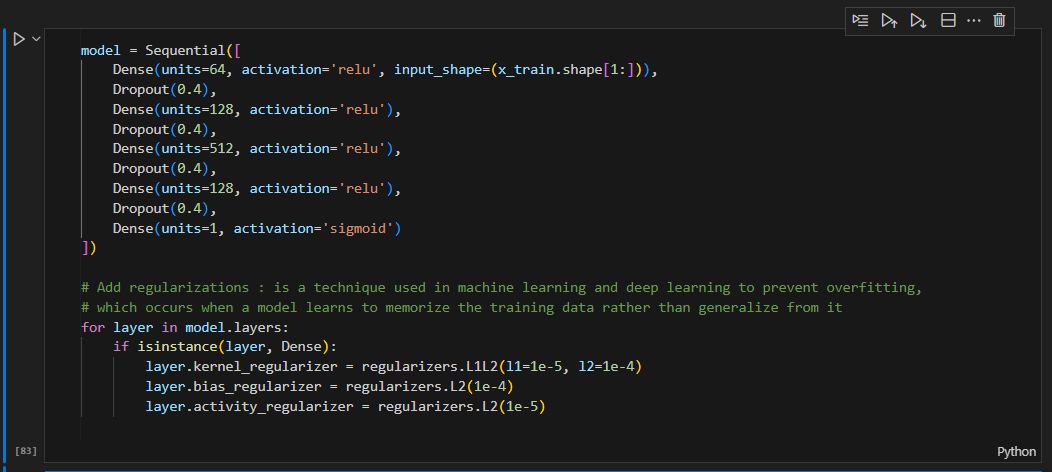
\includegraphics[scale=0.8]{outils-images/data21.png}
\caption{Définir notre modèle DL}
\end{figure}

\noindent \normalsize Pour compile le modèle pour la formation. Il utilise l'optimiseur Adam, un algorithme d'optimisation largement utilisé, ainsi qu'une fonction de perte d'entropie croisée binaire, adaptée aux tâches de classification binaire. De plus, il définit la précision comme mesure permettant d'évaluer les performances du modèle pendant l'entraînement.
\begin{figure}[H]
\centering
 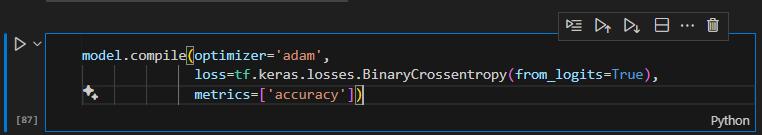
\includegraphics[scale=0.9]{outils-images/data22.png}
\caption{Compile le modèle}
\end{figure}
pour architecture de modèle
\begin{figure}[H]
\centering
 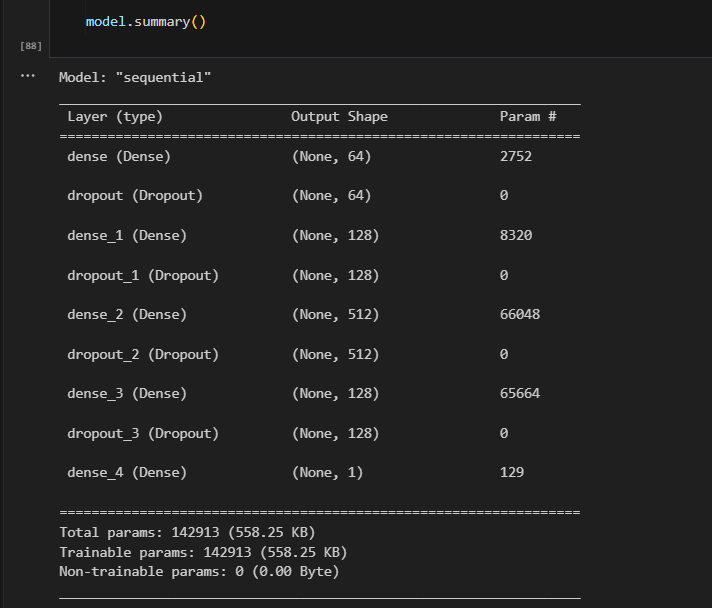
\includegraphics[scale=0.9]{outils-images/data23.png}
\caption{Architecture de modèle}
\end{figure}

\noindent \normalsize Etape suivante est entraîner le modèle compilé en utilisant les données d'entraînement (x-train, y-train). Il valide également les performances du modèle en utilisant les données de validation (x-test, y-test). Pendant l'entraînement, il s'exécute pendant 20 epochs, chaque epoch itérant sur l'ensemble des données. Le paramètre batch-size définit le nombre d'échantillons traités avant la mise à jour des paramètres internes du modèle. De plus, verbose=1 définit le niveau de verbosité de l'entraînement pour afficher des barres de progression pendant l'entraînement. La variable model-train-hist stocke l'historique de l'entraînement, y compris les métriques telles que la perte et la précision, pour une analyse et une visualisation ultérieures
\begin{figure}[H]
\centering
 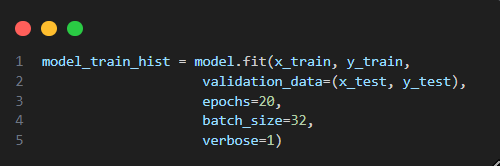
\includegraphics[scale=0.9]{outils-images/data25.png}
\caption{Entraînement notre DL modèle}
\end{figure}
Et comme outputs in terminal on a :
\begin{figure}[H]
\centering
 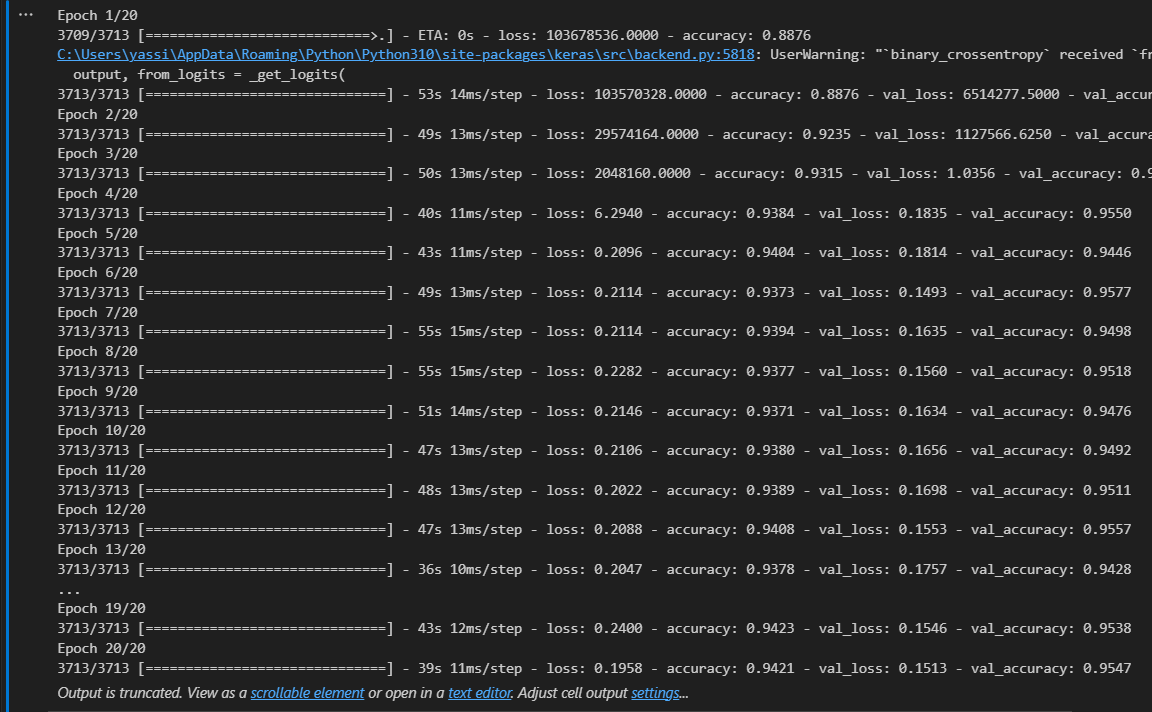
\includegraphics[scale=0.7]{outils-images/data24.png}
\caption{Epochs notre DL modèle}
\end{figure}

\noindent \normalsize Pour évaluation premierment nos tracons les courbes de perte (loss) et de validation (valloss) en fonction du nombre d'epochs. Les données sont extraites de l'historique de l'entraînement model-train-history. Les valeurs sur l'axe des x représentent les epochs, tandis que les valeurs sur l'axe des y représentent la perte (loss) calculée à l'aide de la fonction SCCE Loss (Sparse Categorical Crossentropy). Enfin, le code ajoute des étiquettes d'axe, une légende pour différencier les courbes, et active la grille pour une meilleure lisibilité du graphique
\begin{figure}[H]
\centering
 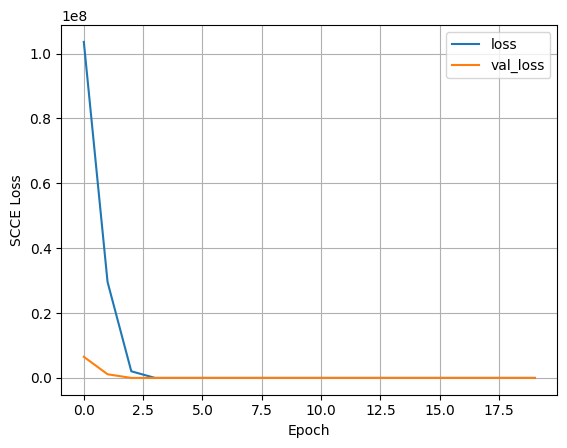
\includegraphics[scale=0.7]{outils-images/graphs/g8.png}
\caption{Epochs en fonction de SCCE Loss}
\end{figure}
Et nous traçons une autre courbe décrivant le changement de l'accuracy à chaque epoch.
\begin{figure}[H]
\centering
 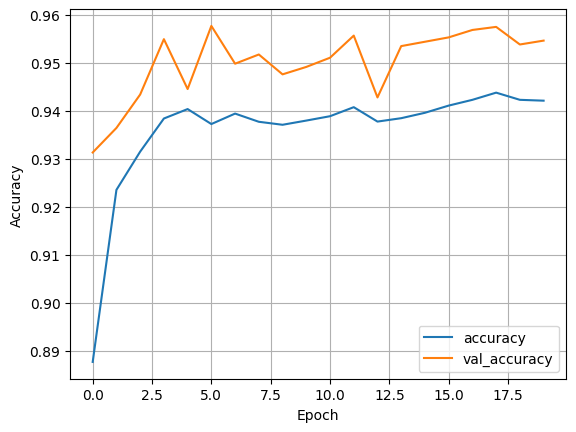
\includegraphics[scale=0.7]{outils-images/graphs/g9.png}
\caption{Epochs en fonction d'accuracy}
\end{figure}
À la fin, nous sauvegardons le modèle dans un fichier ".h5".
\begin{figure}[H]
\centering
 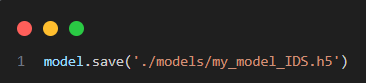
\includegraphics[scale=0.99]{outils-images/data26.png}
\caption{code de sauvegarde le modèle}
\end{figure}

\begin{figure}[H]
\centering
 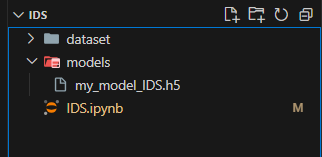
\includegraphics[scale=0.99]{outils-images/data27.png}
\caption{path de sauvegarde}
\end{figure}

\section {Conclusion}
\noindent\normalsize Dans ce chapitre, j'ai décrit tous les aspects possible de notre modèle ainsi que son évaluation.

\chapter*{\centering Conclusion}\addcontentsline{toc}{chapter}{Conclusion}
\noindent\normalsize Ce rapport offre un aperçu du travail réalisé tout au long de mon mini-projet. L'objectif principal était de concevoir un modèle pour un système de détection d'intrusion (IDS) capable de prédire les attaques. J'ai utilisé des technologies modernes pour fournir un code de haute qualité afin de mener à bien ces travaux.\\[0.5cm]
Les différentes étapes qui m'ont été confiées pour accomplir ces tâches comprenaient l'analyse, la conception et le développement. Ce mini-projet a été une excellente occasion pour moi de mettre en pratique les connaissances théoriques acquises lors de ma formation en master en mathématiques, cryptographie et cybersécurité (M2C) à l'École Normale Supérieure de Casablanca.\\[0.5cm]
De plus, mon autoformation m'a permis d'acquérir des compétences dans le travail avec de nouvelles technologies très demandées sur le marché de l'emploi.qualité afin de mener à bien ces travaux.
Pour source code de projet : \href{https://github.com/yassineboujrada/Intrusion_Detection_System_Analyze}{Intrusion Detection System Analyze en Github}.



\bibliographystyle{plain}
\bibliography{sample.bib}

\end{document}
